\section{Model 2}

The results displayed in this section are for the uncertainty involved
in the calculation of flamespeed depending on two parameters: the
activation energy for the fall off reaction in the ozone mechanism and
activation energy for second reaction in the mechanism. The percentage
of ozone is taken as 40, 46, 53, 75, and 100 percent according to the
experimental data available to us from Streng\cite{Streng}.
%% In the
%% figure~\ref{subfig-4:KDE_21}, we display results for sample size 1e7
%% and surrogate of 100X100 points.  We show the the KDE for parameters
%% $E_2$ and $E_3$.


Figure~\ref{subfig-m2-1:E2_sample_conv} and
Figure~\ref{subfig-m2-1:E3_sample_conv} show posterior distributions,
for a constant surrogate size of
$100\times 100$, with varying number of MCMC samples from 1e5 to 1e7. Convergence is observed.
%% The plot is done for raw chain size of $1e5$,
%% $5e5$ , $1e6$, $5e6$ and $1e7$ is taken.
Figure~\ref{subfig-m2-1:E2_surrogate_conv} and
Figure~\ref{subfig-m2-1:E3_surrogate_conv} show the convergence study for
an increasing number of interpolation surrogate points. The number of
surrogate points is varied from $10\times 10$ up to $200\times 200$
for both $E_2$ and $E_3$; the MCMC chain size is
$1e6$.
%% For different starting points of MCMC chain, the MAP point of
%% the resulting pdf does not change. The surrogates for individual
%% concentrations are constructed using linear interpolation
%% function. The initial guess for the MAP point is calculated using
%% Nelder Mead optimization technique.

Figure~\ref{subfig-m2-1:mean_2} and
Figure~\ref{subfig-m2-2:autocorr_2} show mean and autocorrelation
for the samples of the parameters $E_2$ and $E_3$ in order to assess
the required chain thinning.
%% The mean plot shows
%% the initial instability due to sum in period of MCMC and after that it
%% remains constant. It shows us that we should be using at least more
%% than these number of samples for our analysis.
Figure~\ref{subfig-m2-1:e2_distribution_2} and
Figure~\ref{subfig-m2-1:e3_distribution_2} shows the posterior of
$E_2$ and $E_3$, respectively, using the final thinned MCMC chain.
The $E_2$ posterior has the following statistical moments:
Mean: 18.9, Std. Dev.: 4.77, Skewness: -1.38, and Kurtosis: 4.55.
The $E_3$ posterior has the following statistical moments:
Mean: 11.7, Std. Dev.: 7.81, Skewness: -0.743 and Kurtosis: 1.29.


%% The results are displayed in five sections. In first section, the
%% plots are shown for kernel density estimation of parameters $E_3$ and
%% $E_2$. In second section, for constant surrogate size, the number of
%% samples are changed from 1e5 to 1e7 and convergence is observed. In
%% the third part of the results, convergence study is done for
%% surrogates with different sizes. In fourth section, we ensure that
%% samples of the parameter which we are drawing are fitting the
%% flamespeed values of the experiment. In the fifth section mean and
%% correlation plots are shown for the samples of both the
%% parameters. The surrogates for individual concentrations are
%% constructed using linear interpolation function. The initial guess for
%% the map point is calculated using nelder mead optimization
%% technique. After supplying initial guess over large domain it is found
%% that the map point is the same no matter where we start our guess.


 It is necessary to ensure that the samples of the parameter which we
 are drawing are fitting the flamespeed values of the
 experiment. Figure~\ref{subfig-m2-1:40_2} through
 Figure~\ref{subfig-m2-5:100_2} illustrate the calculated flamespeed
 using the generated surrogate models for all the
 parameter samples drawn from the final posterior distribution for
 each parameter.

%\subsection{ Statistics }

% In this section, we display results for sample size 1e7 and surrogate of 100X100 points. We  have plotted the KDE



%\subsection{Convergence Study: Number of Samples }

% In this section, we see the convergence of the probability distribution as we increase the raw chain sample size. The plot is done for surrogate size of 100. In this analysis, raw chain size of $1e5$, $5e5$ , $1e6$, $5e6$ and $1e7$ is taken.




%\subsection{Convergence Study: Surrogate }

%In this section, we see the convergence of the surrogate. As we increase the number of points in the surrogate, results should be close for different surrogate sizes. The plot is done for surrogate size of 10X10, 20X20 30X30 , 100X100, 150X150 and 200X200. In this analysis, raw sample chain size is $1e6$.



%\subsection{Flamespeed data Fit}

 %It is necessary to ensure that the samples of the parameter which we are drawing are fitting the flamespeed values of the experiment. In this section, we calculate the flamespeed for all the parameters drawn using the surrogate generated before. We have taken $1e7$ sample size and calculated flamespeed for different concentrations of ozone.





%\subsection{Mean and Autocorrelation Plots}

%In this section, we show the mean of the samples and autocorrelation plots . The mean plot shows the initial instability due to burning period of MCMC and after that it remains constant. It shows us that we should be using atleast more than these number of samples for our analysis. The last figure shows the histogram and the various parameters of the distribution. For E3: Mean:  11.7, Std. Dev.: 7.81, Skewness:  -0.743 and Kurtosis:  1.29. For E2 stats:Mean:  18.9, Std. Dev.:  4.77, Skewness:  -1.38 and Kurtosis:  4.55.




%% \begin{figure}[H]
%% \centering
%% 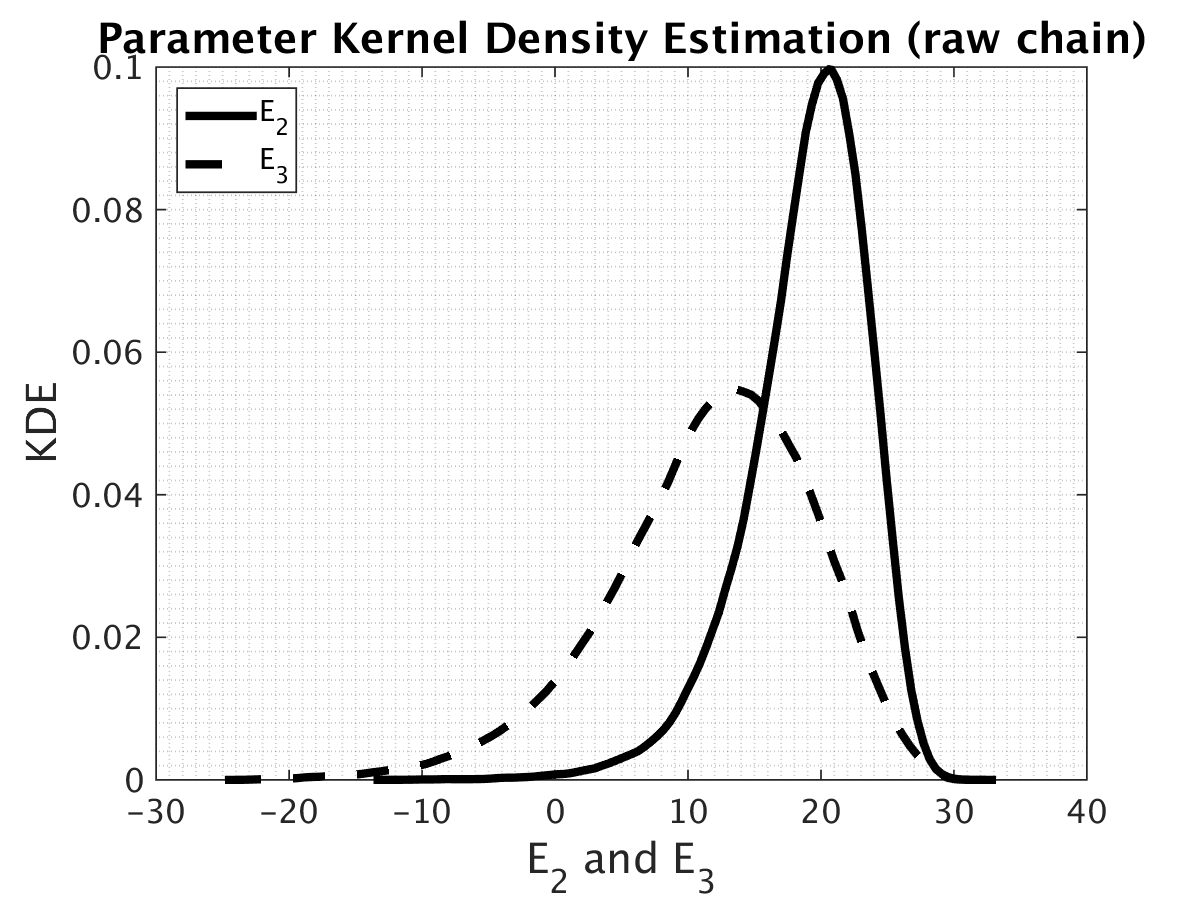
\includegraphics[width=0.45\textwidth]{model_2/kde}
%%    \caption{Posterior distribution for unthinned MCMC chain.}
%%    \label{subfig-m2-4:KDE_21}
%% \end{figure}

 \begin{figure}[H]
   \centering
\subfloat[Convergence For
  $E_2$. \label{subfig-m2-1:E2_sample_conv}]{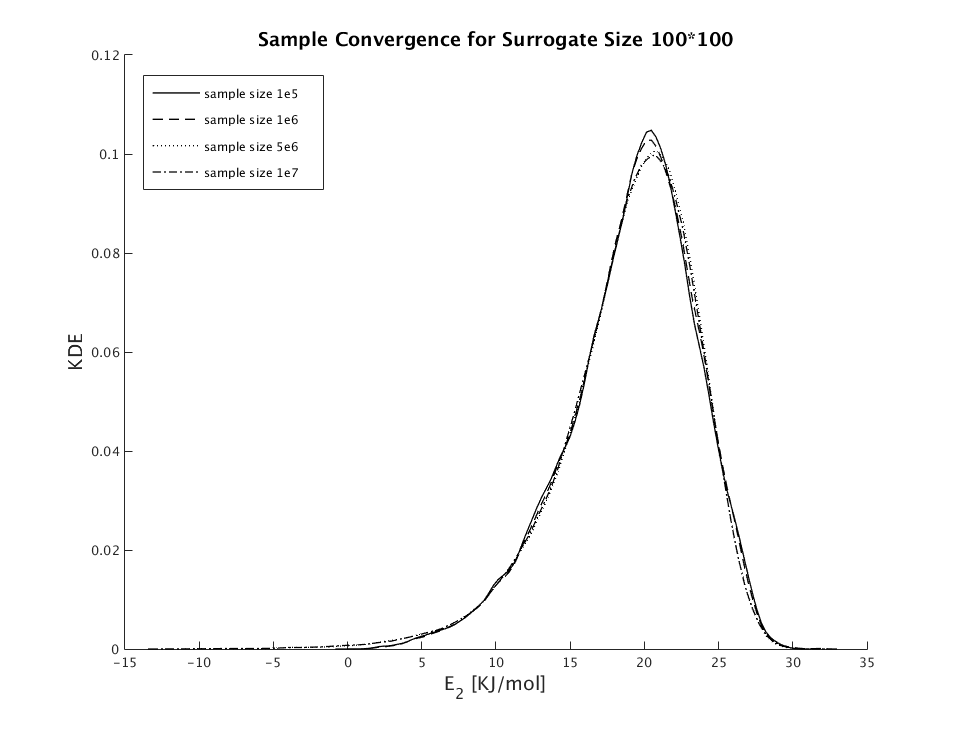
\includegraphics[width=0.45\textwidth]{model_2/sample_conv_E2}}
\subfloat[Convergence For
  $E_3$. \label{subfig-m2-1:E3_sample_conv}]{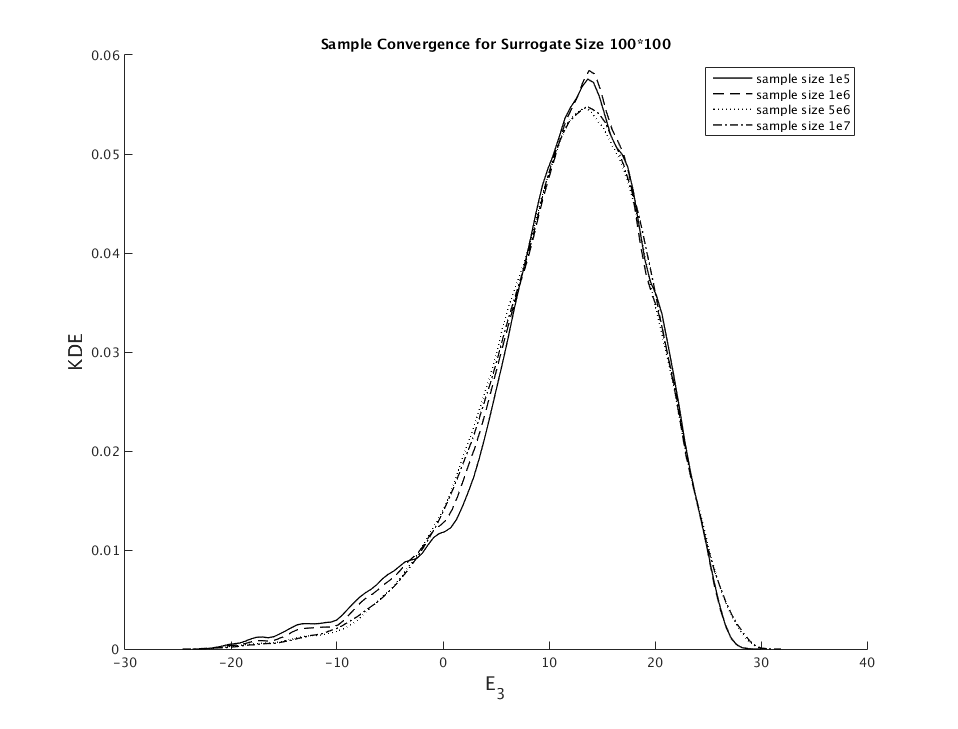
\includegraphics[width=0.45\textwidth]{model_2/sample_conv_E3}}
            \caption{Convergence assessment with respect to increasing
              number of MCMC samples
              for $E_2$ and $E_3$.}
\end{figure}

 \begin{figure}[H]
   \centering
\subfloat[Surrogate Convergence For $E_2$. \label{subfig-m2-1:E2_surrogate_conv}]{
        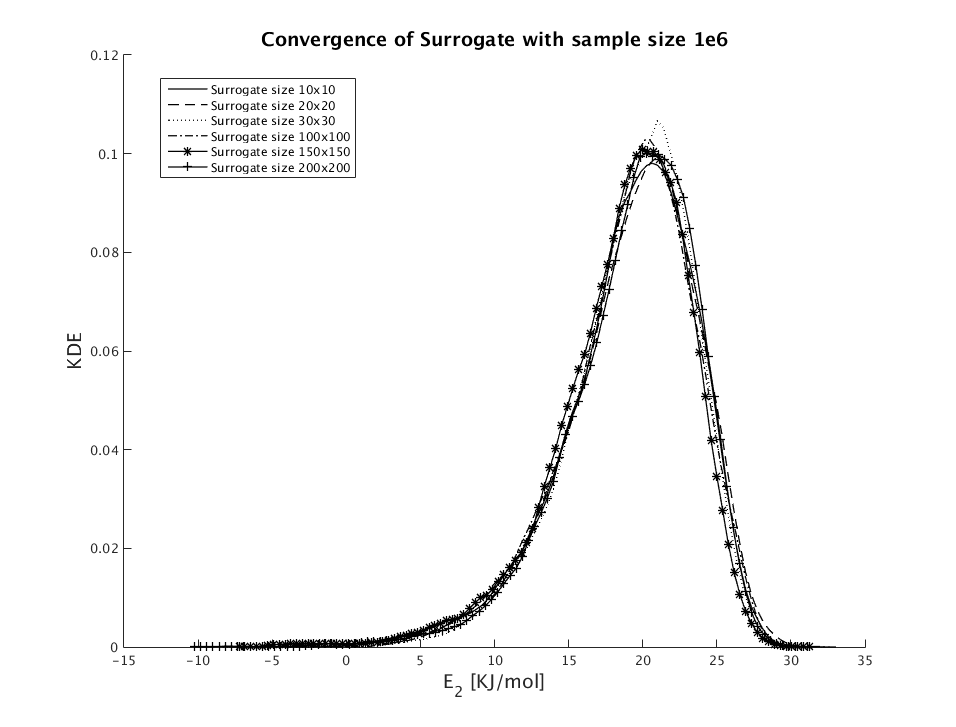
\includegraphics[width=0.45\textwidth]{model_2/surrogate_conv_E2}
            }
 \subfloat[ Surrogate Convergence For $E_3$. \label{subfig-m2-1:E3_surrogate_conv}]{
        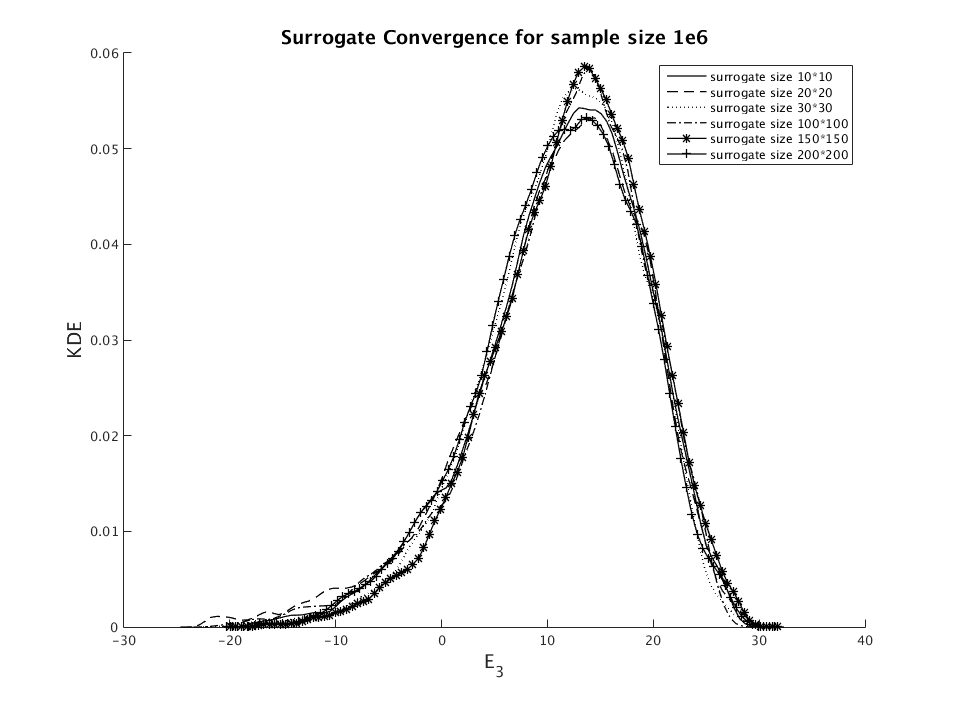
\includegraphics[width=0.45\textwidth]{model_2/surrogate_conv_E3}
            }
            \caption{Convergence with respect to increasing number of
              surrogate evaluations points for $E_2$ and $E_3$. }
\end{figure}




\begin{figure}[H]
  \centering
  \subfloat[ Mean. \label{subfig-m2-1:mean_2}]{
    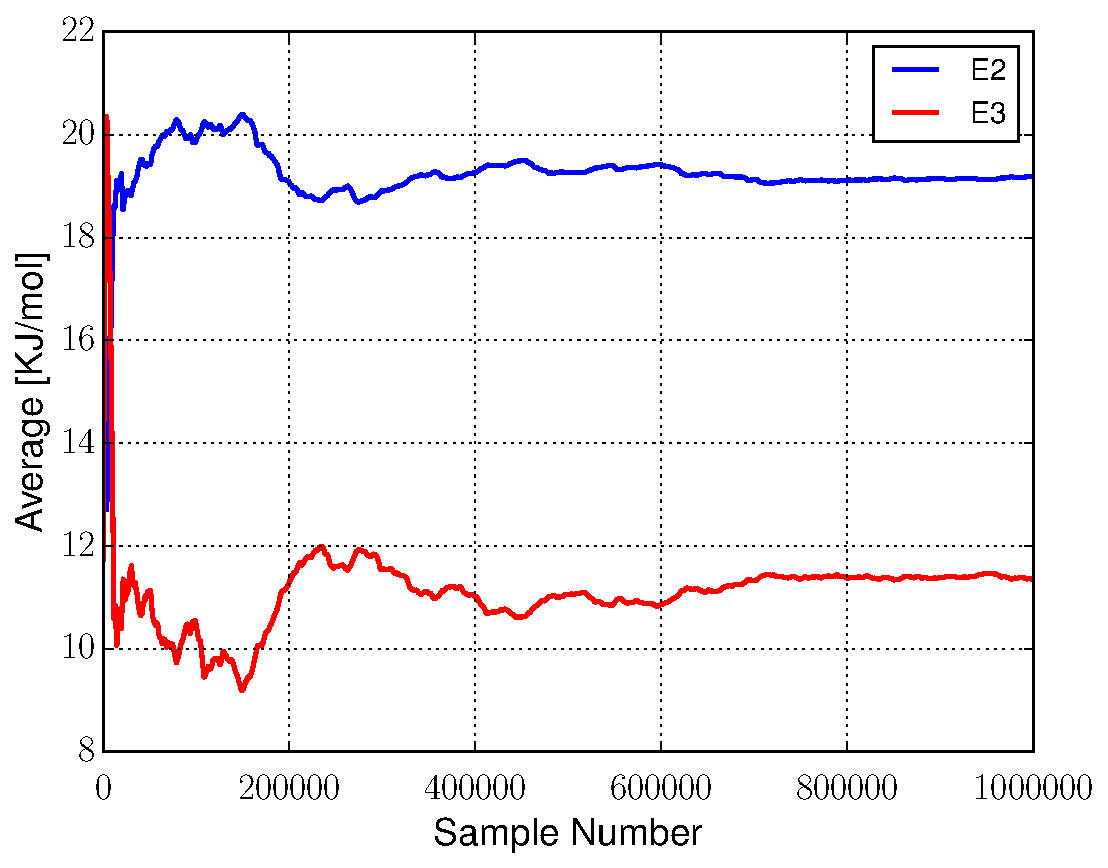
\includegraphics[width=0.45\textwidth]{model_2/M1_running_avg.pdf}
  }
  \subfloat[Autocorrelation. \label{subfig-m2-2:autocorr_2}]{
    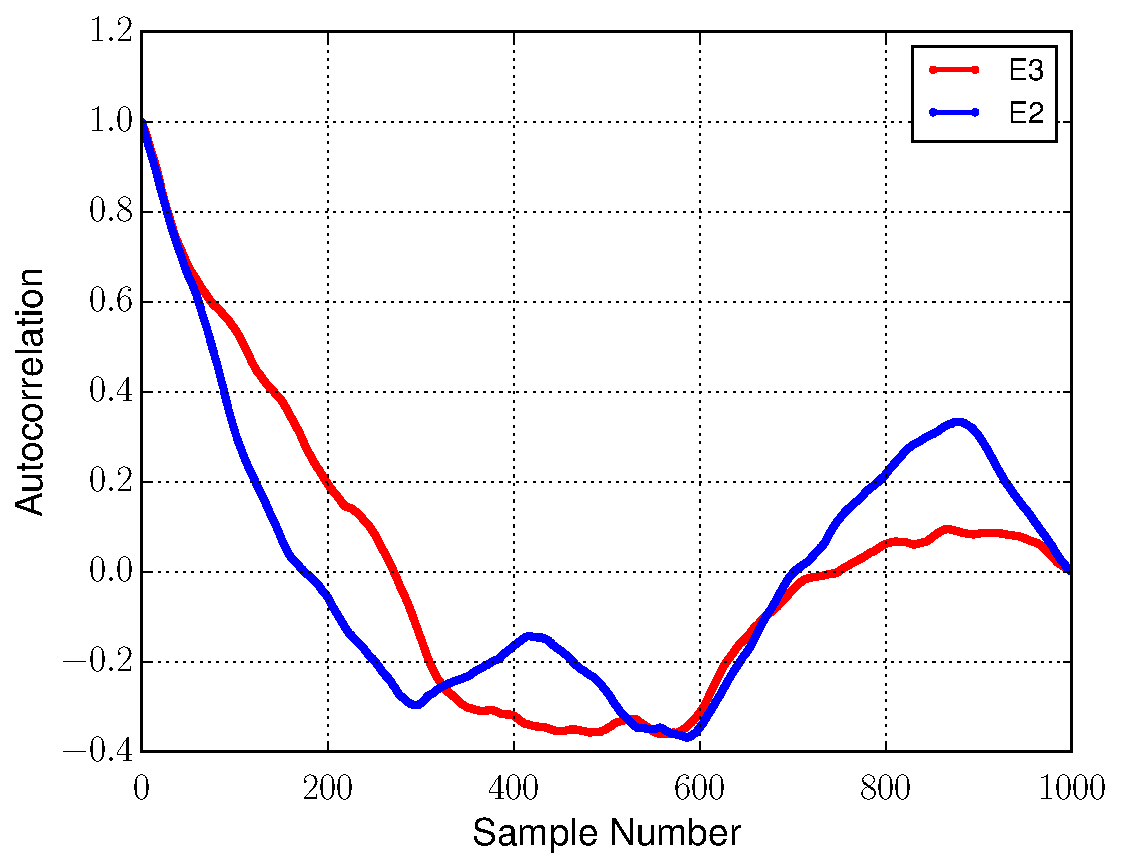
\includegraphics[width=0.45\textwidth]{model_2/M1_autocorr.pdf}
  }
  \caption{Mean and autocorrelation of unthinned MCMC chain.}
\end{figure}

\begin{figure}[H]
  \centering
  \subfloat[  $E_2$ distribution  \label{subfig-m2-1:e2_distribution_2}]{
    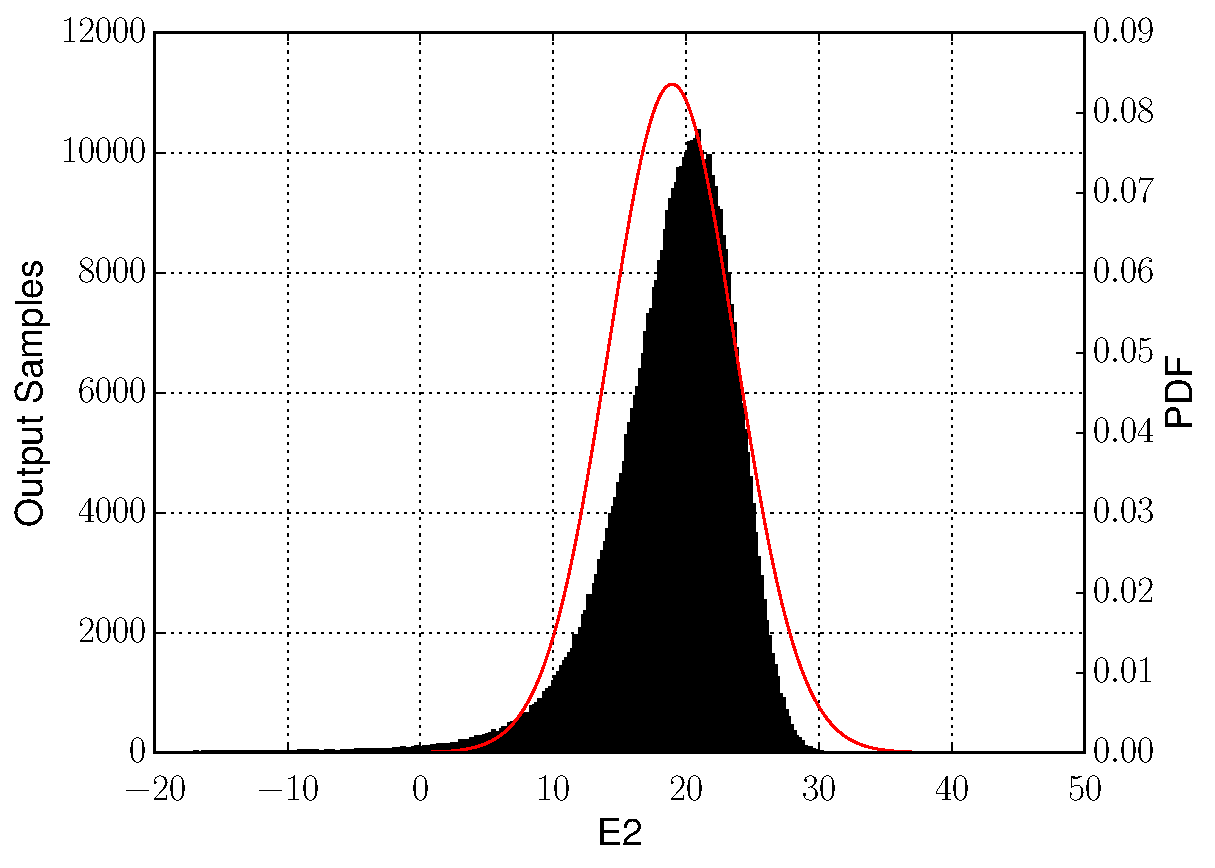
\includegraphics[width=0.45\textwidth]{model_2/E2.pdf}
  }
  \subfloat[ $E_3$ distribution  \label{subfig-m2-1:e3_distribution_2}]{
    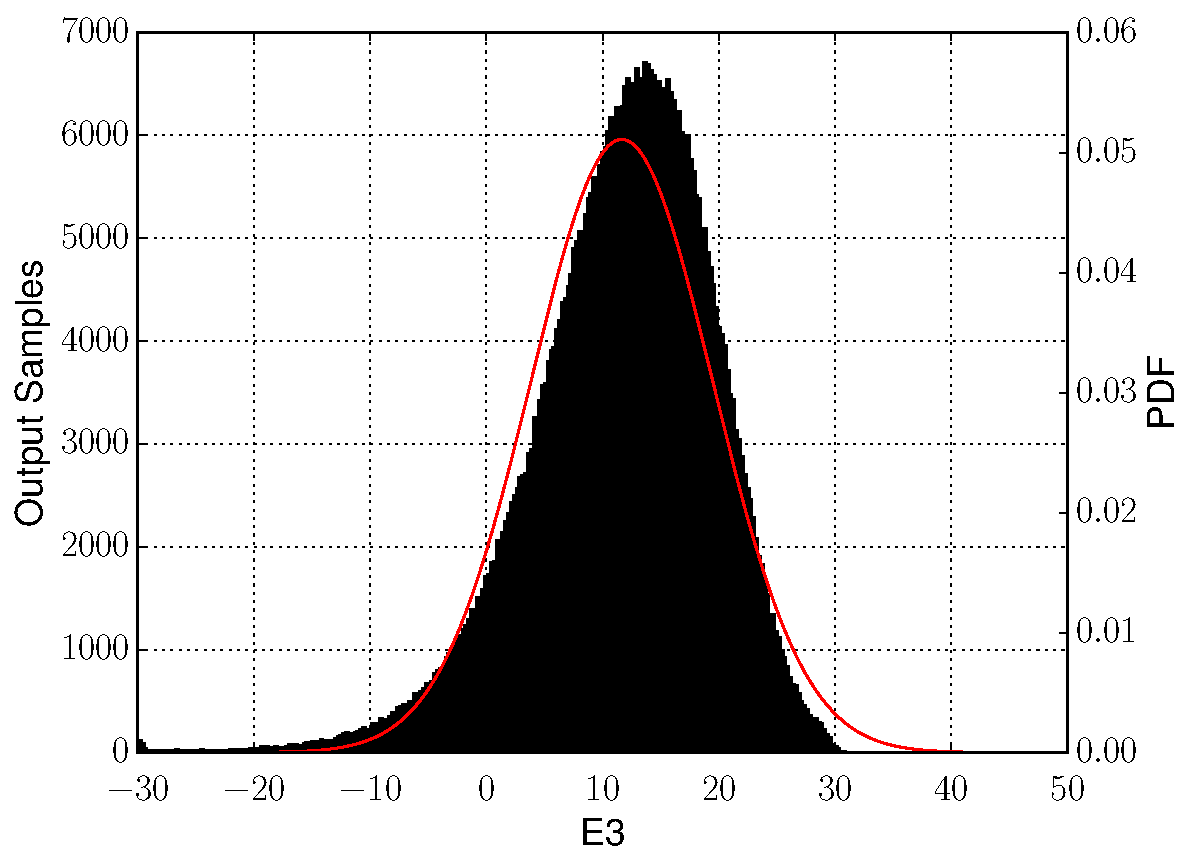
\includegraphics[width=0.45\textwidth]{model_2/E3.pdf}
  }
  \caption{Thinned $E_2$ and $E_3$ posterior distributions. The red curve shows a Gaussian
      generated by mean and standard deviation of samples.}
\end{figure}


 \begin{figure}[H]
   \centering
   \subfloat[ Flame speed for 40 \% ozone. \label{subfig-m2-1:40_2}]{
     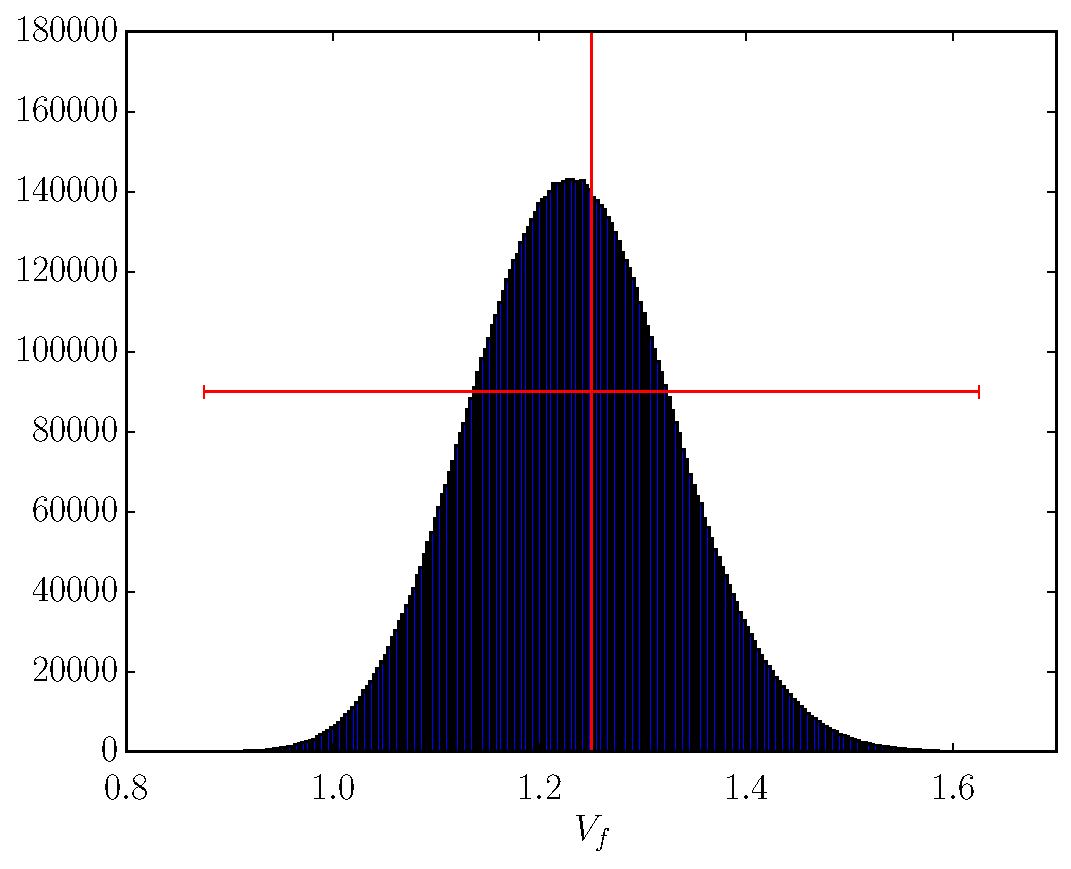
\includegraphics[width=0.45\textwidth]{model_2/flame_40.pdf}
   }
   \subfloat[Flame speed for 46 \% ozone. \label{subfig-m2-2:46_2}]{
     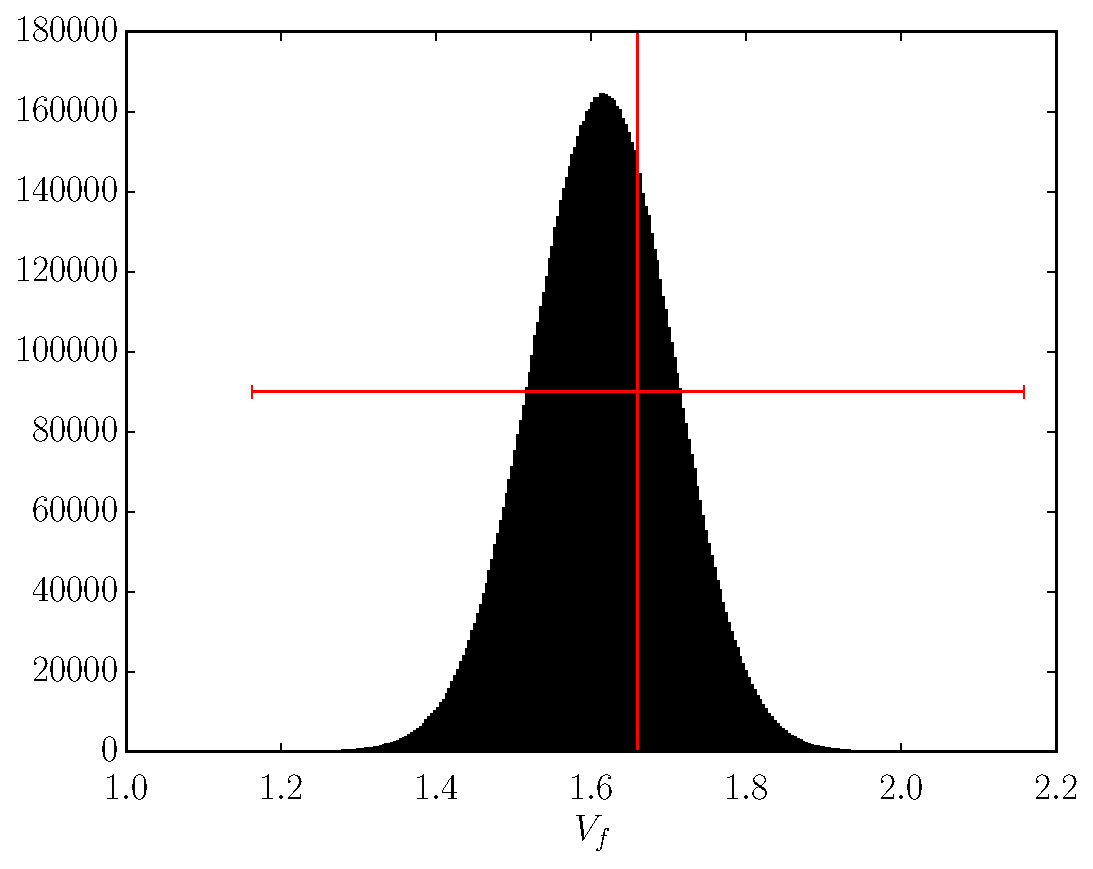
\includegraphics[width=0.45\textwidth]{model_2/flame_46.pdf}
   }

   \subfloat[ Flame speed for 53 \% ozone. \label{subfig-m2-3:53_2}]{
     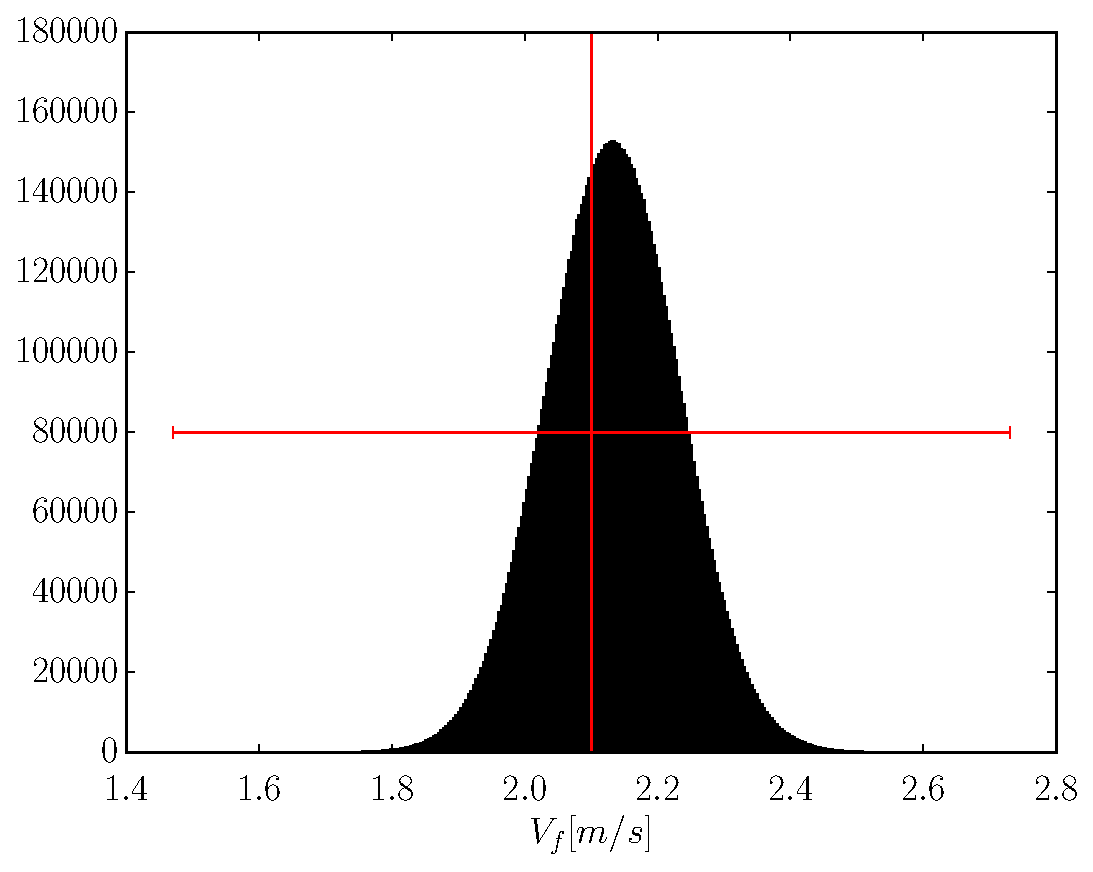
\includegraphics[width=0.45\textwidth]{model_2/flame_53.pdf}
   }
   \subfloat[Flame speed for 75 \% ozone. \label{subfig-m2-4:75_2}]{
     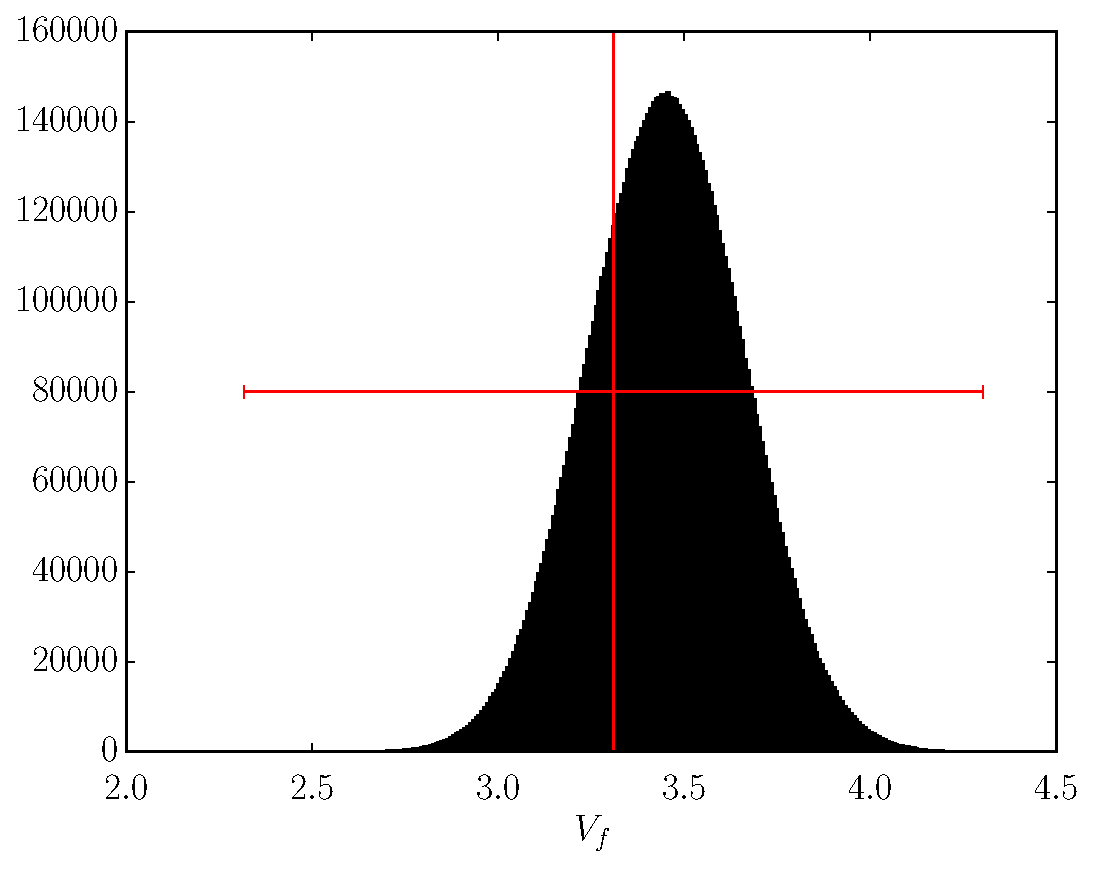
\includegraphics[width=0.45\textwidth]{model_2/flame_75.pdf}
   }

   \subfloat[ Flame speed for 100 \% ozone. \label{subfig-m2-5:100_2}]{
     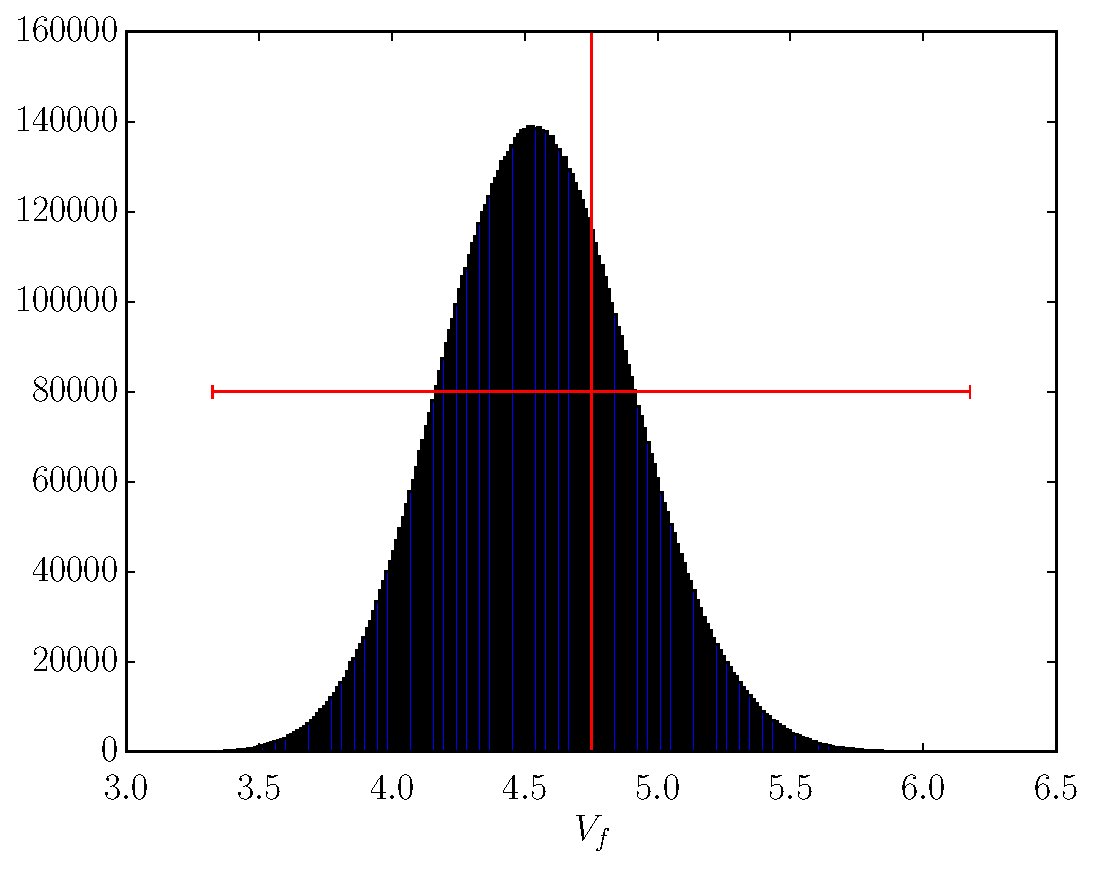
\includegraphics[width=0.45\textwidth]{model_2/flame_100.pdf}
   }
   \caption{Distribution of flamespeed from $E_2$ and $E_3$ posteriors in order to
     assess quality of parameter fit with experimental data. Red
     vertical line is the data value while the horizontal red line is
     $\pm 30\%$.}
 \end{figure}
